\documentclass[dvipdfmx, 10pt]{beamer}
%%%% 和文用 %%%%%
\usepackage{bxdpx-beamer}
\usepackage{pxjahyper}
\usepackage{minijs}%和文用
\renewcommand{\kanjifamilydefault}{\gtdefault}%和文用

%%%%%%%%%%%%%%%%%%%%%%%%%%
%% usepackage 群
%%%%%%%%%%%%%%%%%%%%%%%%%%
\usepackage{amsmath,bm} %多次元空間ベクトルRを表記するのに必要
\usepackage{amsfonts}
\usepackage{ascmac} %枠付き文章を表記するのに必
\usepackage{amssymb}
% \mathbb{R}^{l} %表記例
% \usepackage{algorithm}
% \usepackage{algorithmicx}
% \usepackage{algpseudocode}

%%%% スライドの見た目 %%%%%
\usetheme{Madrid}
\usefonttheme{professionalfonts}

%\useoutertheme[subsection=false]{smoothbars}%ヘッダーにセクション表示
\useinnertheme{circles} % 箇条書きをシンプルに

\setbeamercovered{transparent}%消えている文字をうっすらと表示
\setbeamertemplate{footline}[frame number]%フッターをページ番号だけに
\setbeamerfont{footline}{size=\scriptsize}%ページ番号小さく
\setbeamerfont{frametitle}{size=\large}%フレームタイトルちょい小さく
\setbeamercolor{footline}{bg=black}%ページ番号を太く
\setbeamersize{text margin left=.75zw, text margin right=.75zw}%スライドの横の空白を調節

\setbeamertemplate{enumerate items}[default]%enumerate環境のitemを見やすくする
\setbeamertemplate{section in toc}[square]%outlineのボールを四角に
\setbeamertemplate{navigation symbols}{}%右下のアイコンを消す
%%%%

%%%%%%%%%%%%%%%%%%%%%%%%%%%%%%%%%%%%%%%%%%%%
%%いろいろ便利なもの
%%%%%%%%%%%%%%%%%%%%%%%%%%%%%%%%%%%%%%%%%%%%
\usepackage{here} %[hbtp]の代わりに[H]と書きこむと強制的にその場所に図や表を挿入する
\usepackage{bm}

%%%%%%%%%%%%%%%%%%%%%%%%%%%%%%%%%%%%%%%%%%%%%%%%%
%%newcommand群
%%%%%%%%%%%%%%%%%%%%%%%%%%%%%%%%%%%%%%%%%%%%%%%%%
\newcommand{\argmax}{\mathop{\rm arg~max}\limits}
\newcommand{\argmin}{\mathop{\rm arg~min}\limits}

%%%%%%%%%%%%%%%%%%%%%%%%%%%%%%%%%%%%%%%%%%%%%%%%%
%%本文
%%%%%%%%%%%%%%%%%%%%%%%%%%%%%%%%%%%%%%%%%%%%%%%%%
\title[]{Ridge とLasso の推定}
\author[Y.Omori]{B4 Y.Omori}
\date[\today]{\today}
\institute[NIT]{Nagoya Institute of Technology \\ Takeuchi \& Karasuyama Lab}
% [..]に省略名が書ける

%目次スライド
\AtBeginSection[]{
    \begin{frame}{Next Section}
	\tableofcontents[currentsection, hidesubsections]%目次本体
	%\thispagestyle{empty}%ヘッダーフッター表示なし
	\end{frame}
}

\begin{document}
%タイトル
\begin{frame}{}
\maketitle%タイトル本体
\thispagestyle{empty}%ヘッダーフッター表示なし
\addtocounter{framenumber}{-1}%ページ数カウンタしない
\end{frame}
%目次
\begin{frame}{Outline}
\tableofcontents[hideallsubsections]
\end{frame}

%以降\sectionごとに目次表示
\section{はじめに}
\subsection{正則化法}
\begin{frame}{\insertsubsection}
    \begin{block}{正則化法}
        複雑なモデルの推定において生じる過学習を防ぐ手法
    \end{block}
    \vspace{10pt}
        今回は以下の2つの正則化法を紹介する
    \begin{itemize}
        \item Ridge
      \item Lasso
    \end{itemize}
\end{frame}
\subsection{線形回帰モデル}
\begin{frame}{\insertsubsection}
    次のような線形回帰モデルを考える
    \begin{equation}
    	y_i=\beta_0 + \beta_1 x_{i1} + \beta_2  x_{i2} + \dots + \beta_p x_{ip} + \epsilon_i
    	\label{eq:linear_model_origin}
    \end{equation}    
    \begin{itemize}
        \item $i$番目($i = 1, 2, \dots, n$)のデータの目的変数: $y_i$\\
        \item 説明変数: $\bm{x}_i=(x_{i1}, \dots, x_{ip})^{\top} \in \mathbb{R}^p$\\
        \item 誤差: $\epsilon_i \sim \mathcal{N}(0, \sigma^2)$\\
        \item 回帰係数: $\bm{\beta}=(\beta_0, \beta_1, \dots , \beta_p)^{\top} \in \mathbb{R}^{p+1}$
    \end{itemize}
\end{frame}
\subsection{正則化最小2乗法}
\begin{frame}{\insertsubsection}
    線形回帰モデルに次の正則化項を加える
    \begin{equation}
        S_{\alpha}(\bm{\beta}) = 
        \underset{\text{2乗誤差の和}}{\underline{
            \sum_{i=1}^{n}\bigl(
        		y_i - (
        			\beta_0 + \sum_{j=1}^{p} \beta_j {x}_{ij}
        		)
            \bigr)^2
        }}
    	 +  \underset{\text{正則化項}}{\underline{
            \alpha \sum_{j=1}^{p} |\beta_j|^q
        }}
    	\label{eq:extendLinearRegression}
    \end{equation}
    \begin{itemize}
        \item モデルの複雑度を設定するハイパーパラメータ: $\alpha \in \mathbb{R}^+$
     \end{itemize}
     \vspace{10pt}
    第2項の$q$の値によって次のように呼ばれる
    \begin{enumerate}
        \item $q=1 \rightarrow$ Lasso
        \item $q=2 \rightarrow$ Ridge
    \end{enumerate}
\end{frame}

\section{Ridge とLasso の推定}
\subsection{Ridgeとは}
\begin{frame}{\insertsubsection}
    \begin{block}{Ridge}
        切片を除く回帰係数の2乗和を正則化項としてとることで,説明変数間の強い相関によって生じる回帰係数の推定値の不安定性を回避する手法
    \end{block}
    \vspace{10pt}
    Ridge推定量を導出するため,線形回帰モデルの中心化を考える
    \begin{equation}
        y_i = \beta_0^* + \beta_1 z_{i1} + \dots + \beta_p z_{ip} + \epsilon_i
	\label{eq:linear_model_centering}
    \end{equation}
    \begin{itemize}
    	\item $j$番目の説明変数に関するデータの平均値: $\bar{x}_j$
	\item  $\bar{x}_j$を中心化したデータ: $z_{ij}=x_{ij} - \bar{x}_j$
	\item $\beta_0^* = \beta_0 + \beta_1 \bar{x}_{1} + \dots + \beta_p \bar{x}_{p}$
    \end{itemize}
\end{frame}
\subsection{Ridge回帰モデル}
\begin{frame}{\insertsubsection}
    中心化した線形回帰モデルは次の行列形式で記述できる
    \begin{equation}
	\begin{split}
		\bm{y} &= \beta_0^* \bm{1} + Z \bm{\beta}_1 + \bm{\epsilon}\\
		Z &= \left[
                \begin{array}{ccc}
                z_{11} & \dots & z_{1p} \\
                \vdots & z_{ij} & \vdots \\
                z_{n1} & \dots & z_{np} \\
                \end{array}
                \right]
        \end{split}
	\label{eq:linear_model_mat}
    \end{equation}
    \begin{itemize}
    	\item $\bm{\beta}_1 = (\beta_1, \beta_2, \dots , \beta_p)^{\top} \in \mathbb{R}^p$
	\item $ \bm{1} = (1, 1, \dots , 1)^{\top} \in \mathbb{R}^n$
    \end{itemize}
    \vspace{10pt}
    以上よりRidge回帰モデルは次の式となる
    \begin{equation}
        	S_{\alpha}(\beta_0^* , \bm{\beta}_1) = (\bm{y} - \beta_0^* \bm{1} - Z \bm{\beta}_1)^{\top} (\bm{y} - \beta_0^* \bm{1} - Z \bm{\beta}_1) + \alpha \bm{\beta}_1^{\top} \bm{\beta}_1 
    	\label{eq:ridge_estimate}
    \end{equation}
    \vspace{10pt}
    この式の最小化により次のような切片と回帰係数ベクトルの推定量が与えられる
\end{frame}
\subsection{Ridgeの推定量}
\begin{frame}{\insertsubsection}
	中心化したRidge回帰モデルの推定量
	\begin{itemize}
	\item 切片: $\hat{\beta_0^*} = \bar{y} = \frac{\sum_{i=1}^{n}{y_i}}{n}$
	\item 回帰係数ベクトル: $\hat{\bm{\beta}_1} = (Z^{\top}Z + \alpha I_p)^{-1} Z^{\top} \bm{y}$
	\end{itemize}
    \vspace{10pt}
    この結果から式\eqref{eq:linear_model_origin}の切片は$\hat{\beta_0} = \bar{y} - \hat{\beta}_1 \bar{x}_1 - \dots - \hat{\beta_p} \bar{x}_p$と推定される\\
    \vspace{10pt}
    $\rightarrow$ \quad $\beta_0^*$を考えることなく
\begin{equation}
	S_{\alpha}(\bm{\beta}_1) = (\bm{y} - Z \bm{\beta}_1)^{\top}  (\bm{y} - Z\bm{\beta}_1) + \alpha \bm{\beta}_1^{\top} \bm{\beta}_1
	\label{eq:ridge_estimate_beta1hat}
\end{equation}
の最小化によって$\hat{\bm{\beta}_1}$を得られる
\end{frame}

\subsection{Lassoとは}
\begin{frame}{\insertsubsection}
    \begin{block}{Lasso}
        切片を除く回帰係数の絶対値の和を正則化項としてとることで,パラメータの一部は完全に0になることから,モデルの推定と変数選択を同時に実行できる手法
    \end{block}
    \vspace{10pt}
    切片を除く回帰係数はデータの中心化によって切片と切り離して推定できる\\
    $\rightarrow$次の式の最小化によって与えられる
    \begin{equation}
        S_{\alpha}(\bm\beta_1) = \sum_{i=1}^{n} \bigl(
        	y_i - \sum_{j=1}^{p} \beta_j z_{ij}
        \bigr)^2 + \alpha \sum_{j=1}^{p}|\beta_j|
    \end{equation}
\end{frame}
\subsection{Lassoの計算手法}
\begin{frame}{\insertsubsection}
    $L_1$正則化項が微分不可能であるため解析的に$\bm{\beta}_1$を求めることはできない\\
    $\rightarrow$ 次のような計算手法が用いられる
    \begin{itemize}
	\item shootingアルゴリズム (Fu 1998)
	\item LARS (Efron et al. 2004)
    \end{itemize}
	\vspace{10pt}
	また,ラグランジュの未定乗数法を用いて制約つき最小化問題に変形できる
	\begin{equation}
        	\min \sum_{i=1}^{n}\bigl(
        		 y_i - \sum_{j=1}^{p} \beta_j z_{ij}
        	\bigr)^2 \quad
        	\text{subject to} \quad \sum_{j=1}^{p} |\beta_j| \leq \eta
        \end{equation}

\end{frame}

\section{計算機実験}
\subsection{実験の設定}
\begin{frame}{\insertsubsection}
    通常の最小2 乗法,Ridge およびLasso を用いて回帰係数の推定を行った
    \begin{block}{実験設定}
        \begin{itemize}
                \item 目的変数: アメリカのボストン州の住宅価格
                \item 説明変数: 住宅価格に影響を与えていると思われる以下の13個
                    \begin{table}[htb]
                    	\begin{tabular}{ll}
                    	$x_1$: 犯罪率  & $x_2$: 宅地の割合\\
                    	$x_3$: 非商用地 &  $x_4$: チャールズ川流域か否か\\
                    	$x_5$: 窒素酸化物 &  $x_6$: 部屋数\\
                    	$x_7$: 築年 &  $x_8$: ビジネス地域への距離\\
                    	$x_9$: ハイウェイアクセス指数 &  $x_{10}$: 固定資産税\\
                    	$x_{11}$: 生徒と教師の比率 &  $x_{12}$: 有色人種の割合\\
                    	$x_{13}$: 低所得者の割合\\
                    	\end{tabular}
                    \end{table}
                \item データ数: 506
        \end{itemize}
    \end{block}
\end{frame}

\subsection{正則化の確認}
\begin{frame}{\insertsubsection}
    \begin{figure}[H]
            \begin{tabular}{ccc}
            	\begin{minipage}{0.33\hsize}
                    	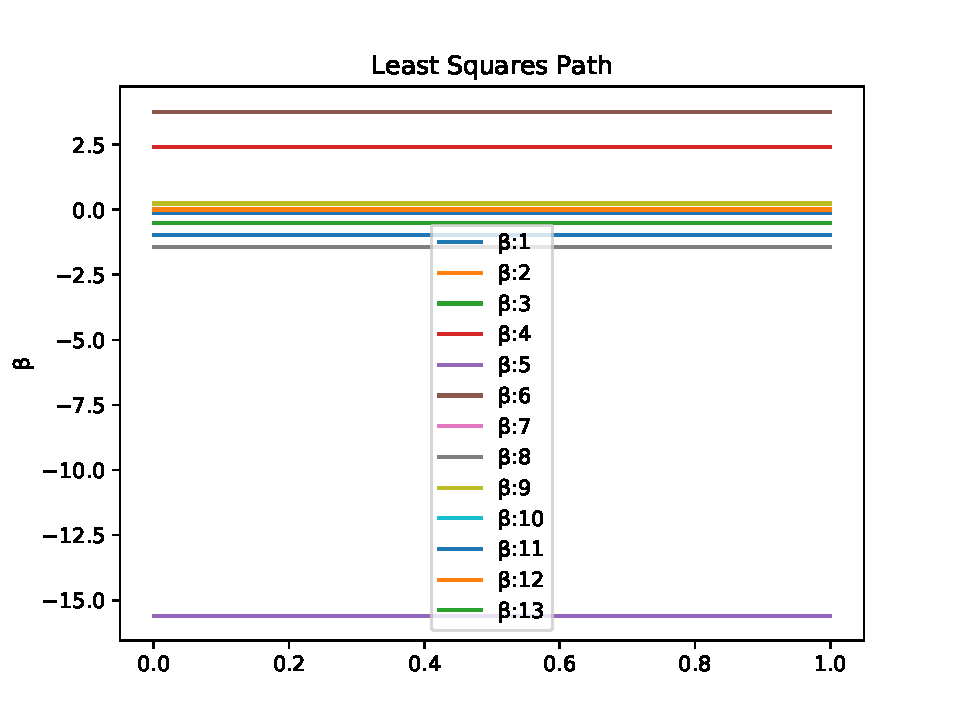
\includegraphics[width=1.0\linewidth]{../img/lrPath.pdf}
                    	\caption{最小2乗法の推定値}
                   	\label{fig:lr}
            	 \end{minipage}
            	 \begin{minipage}{0.33\hsize}
                   	 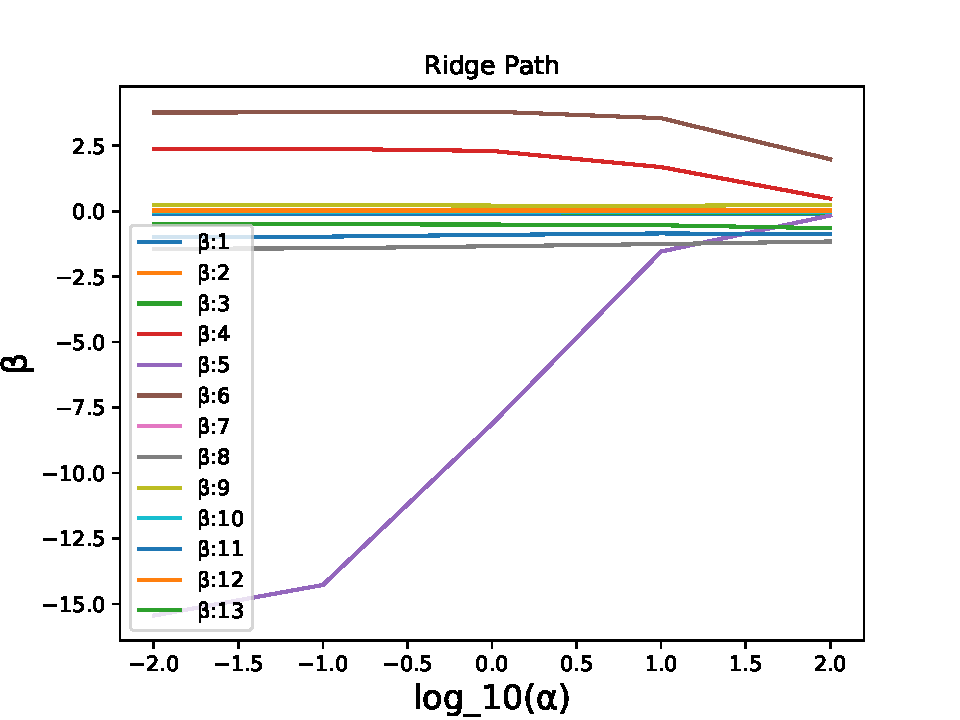
\includegraphics[width=1.0\linewidth]{../img/ridgePath.pdf}
            		 \caption{Ridgeの解パス}
            		 \label{fig:ridge}
            	 \end{minipage}
            	 \begin{minipage}{0.33\hsize}
                   	 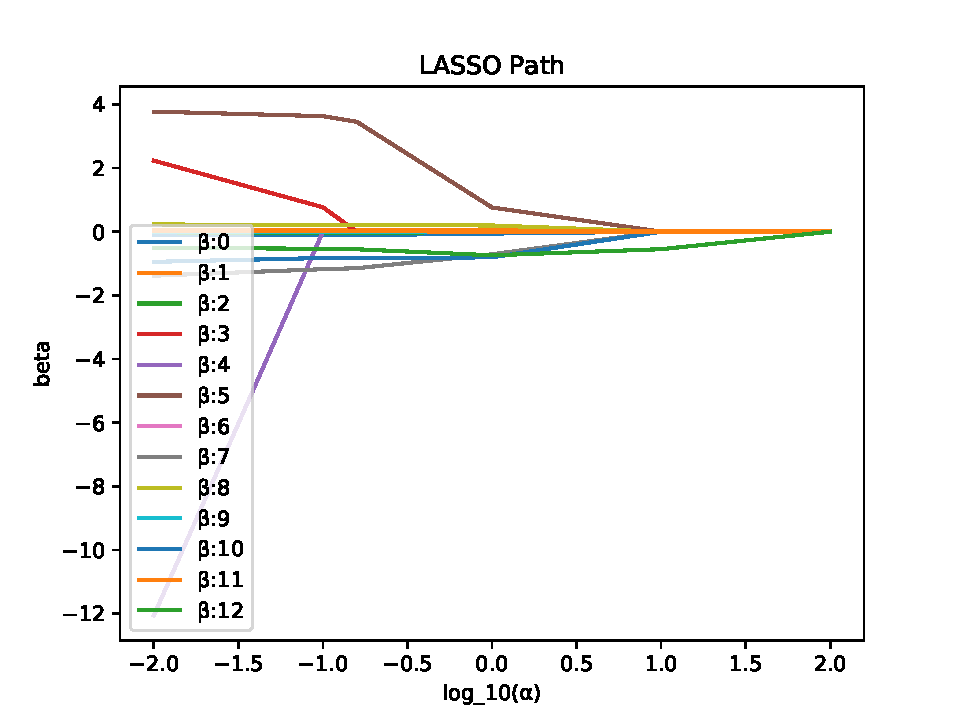
\includegraphics[width=1.0\linewidth]{../img/lassoPath.pdf}
            		 \caption{Lassoの解パス}
            		 \label{fig:lasso}
            	 \end{minipage}
    	     \end{tabular}
    \end{figure}
    \begin{itemize}
        \item $\alpha$が0に近いほど,RidgeとLassoの各推定値は最小2乗法のそれに近い
        \item $\alpha$が大きくなるにつれて,RidgeもLassoも全説明変数の推定値が0に向かって縮小
         \begin{itemize}
            \item 特に,Lassoにおいて$\alpha$=100の場合は全ての回帰係数の値がほぼ0
         \end{itemize}
    \end{itemize}
    $\rightarrow$ $\alpha$の大きさの違いによって正則化の強さが変化することを確認できる
\end{frame}

\subsection{Lassoの変数選択の確認}
\begin{frame}{\insertsubsection}
    \begin{figure}[H]
            \begin{tabular}{cc}
            	 \begin{minipage}{0.5\hsize}
                   	 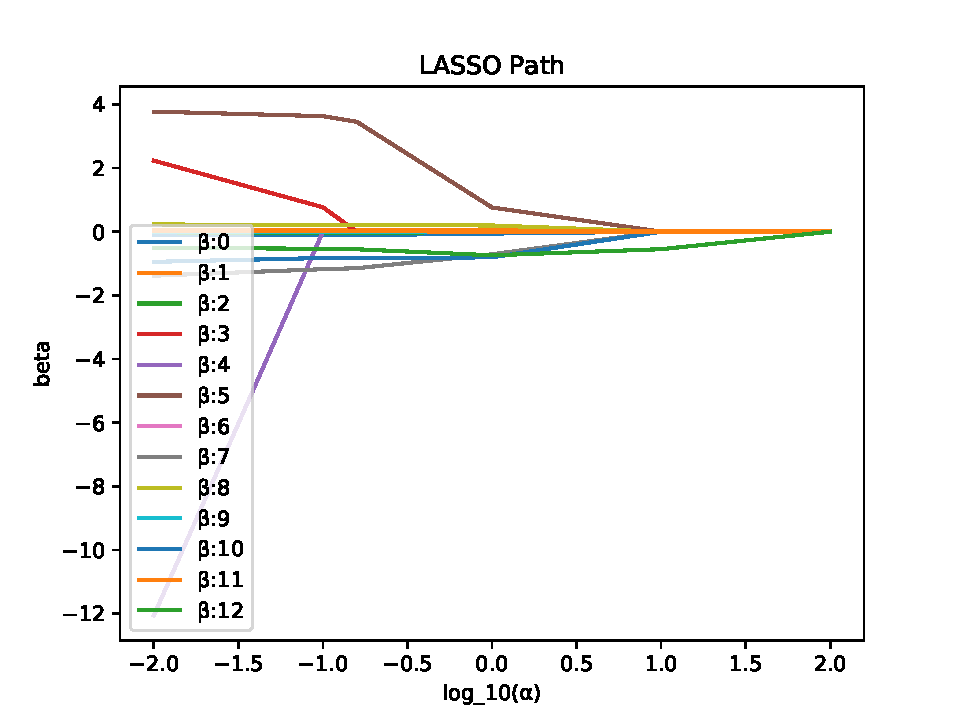
\includegraphics[width=1.0\linewidth]{../img/lassoPath.pdf}
            		 \caption{Lassoの解パス}
            		 \label{fig:lasso}
            	\end{minipage}
	 	\begin{minipage}{0.5\hsize}
                           左図から変数選択の結果が確認できる
                               \begin{itemize}
                                   \item $\alpha=100$において選択された変数
                                    \begin{itemize}
                                        \item 固定資産税($x_{10}$)
                                        \item 有色人種の割合($x_{12}$)
                                   \end{itemize}
                                  \item $\alpha=10$において選択された変数
                                  \begin{itemize}
                                        \item $x_{10}$と$x_{12}$
                                        \item 宅地の割合($x_2$)
                                        \item 低所得者の割合($x_{13}$)
                                   \end{itemize}
                               \end{itemize}
            	\end{minipage}
    	     \end{tabular}
    \end{figure}
    \end{frame}

\subsection{決定係数の実験設定}
\begin{frame}{\insertsubsection}
    推定手法の精度を比較するため,説明変数の数を103に増やして実験
    \begin{block}{実験設定}
        \begin{itemize}
                \item 目的変数: アメリカのボストン州の住宅価格
                \item 説明変数: 住宅価格に影響を与えていると思われる103個
                \item データ数: 506
        \end{itemize}
    \end{block}
    推定手法の精度の指標として決定係数$R^2$を用いた
    \begin{equation}
    	R^2 = 1 - \frac{\sum_{i}^{}(y_i - \hat{y}_i)^2}{\sum_{i}^{}(y_i - \bar{y})^2}
    \end{equation}
\end{frame}

\subsection{決定係数の実験結果}
    \begin{frame}{\insertsubsection}
       \begin{figure}[H]
        \begin{tabular}{ccc}
    	 \begin{minipage}{0.4\hsize}
                    	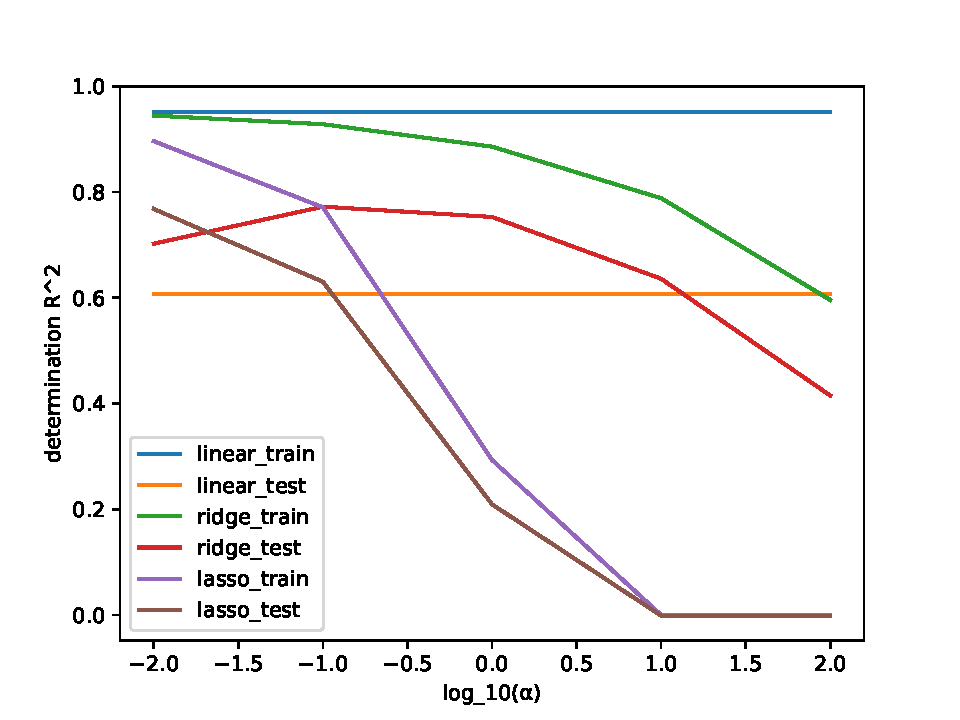
\includegraphics[width=1.0\linewidth]{../img/score.pdf}
                    	\caption{決定係数の推移}
                   	\label{fig:score}
              \end{minipage}
    	 \begin{minipage}{0.6\hsize}
                	 \begin{table}[H]
                        	\centering
                        	\caption{決定係数の結果表}
                                	\begin{tabular}{|c|c|c|c|c|c|}
                        		\hline
                                		$\alpha$ & 0.01 & 0.1 & 1 & 10 & 100\\ 
                        		\hline
                        		\hline
                        		\multicolumn{6}{|c|}{train} \\
                        		\hline
                        		linear & \multicolumn{5}{|c|}{0.95} \\
                        		\hline
                        		ridge & 0.94 & 0.93 & 0.89 & 0.79 & 0.60 \\
                        		\hline
                        		lasso & 0.90 & 0.77 & 0.29 & 0.00 & 0.00\\
                        		\hline
                        		\hline
                        		\multicolumn{6}{|c|}{test} \\
                        		\hline
                        		linear & \multicolumn{5}{|c|}{0.61} \\
                        		\hline
                        		ridge & 0.70 & 0.77 & 0.75 &0.64 & 0.42\\
                        		\hline
                        		lasso & 0.77 & 0.63 & 0.21 & 0.00 & 0.00 \\
                        		\hline
                                	\end{tabular}
                        	\label{tab:score}
                    \end{table}
             \end{minipage}
    	\end{tabular}
    \end{figure}
    \begin{itemize}
        \item 訓練データ
         \begin{itemize}
            \item $\alpha$が大きくなるにつれて,両方の決定係数が減少
        \end{itemize}
       \item テストデータ
         \begin{itemize}
            \item 適切な$\alpha$を設定することで,両方において最小2乗法を上回る精度を出す
        \end{itemize}
    \end{itemize}
\end{frame}

\section{まとめ}
\begin{frame}{\insertsection}
    
    \begin{itemize}
        \item RidgeとLassoを中心に,正則化法や線形回帰モデルについて学習できた
        \item 数式だけでなく,Pythonのパッケージを用いた計算機実験による可視化を通して,自分の中でさらにイメージを具体化させることができた
        \item 今後は,Lassoの計算に用いるアルゴリズムを理解して,パッケージを使わずに実装することが課題である
    \end{itemize}
\end{frame}

\section*{参考文献 (References)}
\begin{frame}{\insertsection}
    \begin{enumerate}
        \item 小西貞則, 『多変量解析入門』. 岩波書店, 2009.
    \end{enumerate}
\end{frame}

\end{document}